% Created 2025-02-11 Tue 16:01
% Intended LaTeX compiler: pdflatex
\documentclass[11pt,oneside]{memoir}
\makeatletter

\usepackage{answerkey-env}

\ifanswerkey
  \usepackage[forcolorpaper, answerkey]{eqexam}
  \usepackage{vinaya-class-questions}
\else
  \usepackage[forcolorpaper, nosolutions]{eqexam}
  \usepackage[nosolutions]{vinaya-class-questions}
\fi

\proofingsymbolColor{linkred}
\fillinColor{linkred}

\def\maketitle{}

\maxtocdepth{subsection}

\newenvironment{twocols}{%
  \raggedright%
  \setlength{\parindent}{0pt}%
  \setlength{\parskip}{8pt}%
  \fontsize{11}{17}\selectfont%
  \begin{multicols}{2}%
}{%
  \end{multicols}%
}

\newenvironment{widecols}{%
  \hspace*{-0.05\linewidth}\begin{minipage}{1.1\linewidth}%
  \raggedright%
  \setlength{\parindent}{0pt}%
  \setlength{\parskip}{8pt}%
  \fontsize{11}{17}\selectfont%
  \begin{multicols}{2}%
}{%
  \end{multicols}%
  \end{minipage}%
}

\newlength\@tmp@width
\newlength\@tmp@height

\renewcommand*{\printchaptertitleHook}{%
  \AddToShipoutPictureBG*{%
    \put(\LenToUnit{\paperwidth-25mm-\spinemargin},\LenToUnit{\paperheight-95mm}){%
      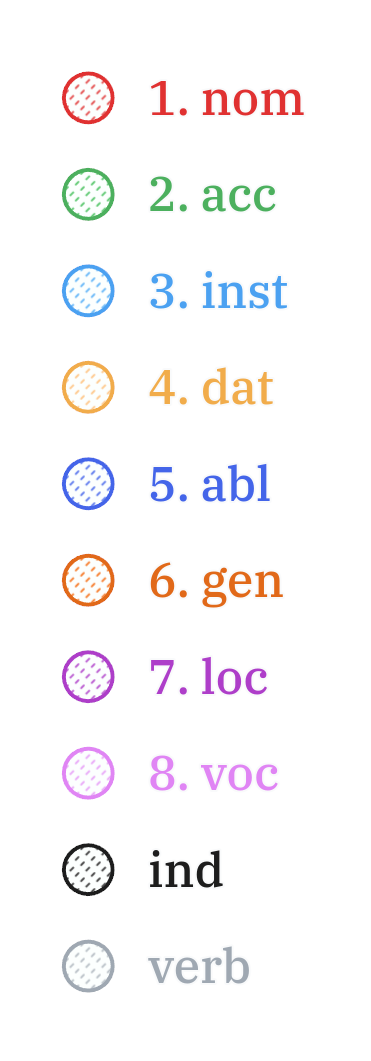
\includegraphics[width=25mm]{./images/cases-legend-white-large.png}%
    }%
  }%
}

\newcommand*\sentenceDiaMsg{\textbf{Exercise:} Draw a sentence analysis diagram below and indicate declensions.}

\newcommand*\sentenceDiaSolution[2][0.4]{%
  \ifanswerkey%
    \hspace*{-\spinemargin}%
    \begin{minipage}{\paperwidth}%
      \centering%
      \includegraphics[scale=#1]{#2}%
    \end{minipage}%
  \else%
    \settototalheight{\@tmp@height}{\includegraphics[scale=#1]{#2}}%
    \begin{minipage}[\@tmp@height]{\linewidth}%
      \sentenceDiaMsg%
    \end{minipage}%
  \fi%
}

\usepackage{cwpuzzle}

\renewcommand\PuzzleCluePre{%
  \begin{minipage}[t]{0.75\linewidth}%
}

\renewcommand\PuzzleClueFont{\fontsize{11}{17}\selectfont}

% \def\PuzzleThickline{\linethickness{2pt}}

\makeatother

\maxtocdepth{section}
\date{\today}
\title{Pāli Readings}
\hypersetup{
 pdfauthor={The Bhikkhu Saṅgha},
 pdftitle={Pāli Readings},
 pdfkeywords={},
 pdfsubject={},
 pdfcreator={Emacs 29.4 (Org mode 9.6.15)}, 
 pdflang={En_Gb}}
\begin{document}

\maketitle
\makeatletter

\newlength{\colOne}\setlength{\colOne}{0.35\linewidth}
\newlength{\colTwo}\setlength{\colTwo}{0.6\linewidth}

\renewenvironment{quote}%
{\list{}{%
    \doubleLineSize
    \listparindent 0pt
    \itemindent    0pt
    \leftmargin    3em
    \rightmargin   3em
    \parsep        0pt
    \topsep        8pt
    \partopsep     0pt}%
\item[] \raggedright}%
{\endlist}

\renewcommand*{\printchaptertitleHook}{%
  \AddToShipoutPictureBG*{%
    \put(\LenToUnit{\paperwidth-25mm-\spinemargin},\LenToUnit{\paperheight-100mm}){%
      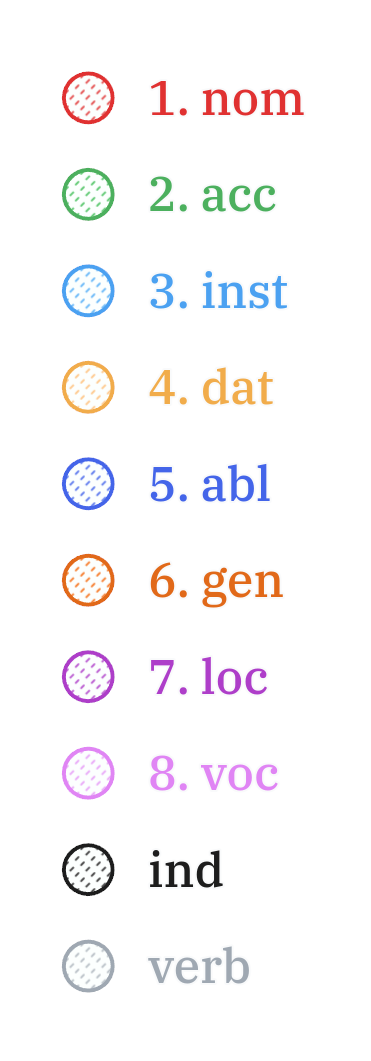
\includegraphics[width=25mm]{./images/cases-legend-white-large.png}%
    }%
  }%
}

\renewcommand*\sentenceDiaSolution[2][0.4]{%
  \ifanswerkey%
    \hspace*{-\spinemargin}%
    \begin{minipage}{\paperwidth}%
      \centering%
      \includegraphics[scale=#1]{#2}%
    \end{minipage}%
  \fi%
}

\makeatother

\mainmatter

\chapter{2025-02-13}
\label{sec:orgdd07a5d}
\section{MN 74 Commentary, a spontaneous gathering of 1250 arahants}
\label{sec:org4ccabb7}
(\href{https://www.digitalpalireader.online/\_dprhtml/index.html?loc=m.1.2.0.0.3.0.a\&para=23}{DPR}, \href{http://localhost:4848/suttas/s0202a.att/pli/cst4?quote=ve\%25E1\%25B8\%25B7uvana\%25E1\%25B9\%2581\%2520gantv\%25C4\%2581\%2520s\%25C4\%2581vakasannip\%25C4\%2581tamak\%25C4\%2581si\&window\_type=Sutta+Study}{SSP}) Dīghanakhasutta-vaṇṇanā

\vspace*{-\baselineskip}

\begin{quote}
Bhagavā pana imaṁ desanaṁ sūriye dharamāne'yeva niṭṭhāpetvā

gijjhakūṭā oruyha veḷuvanaṁ gantvā sāvakasannipātam'akāsi,

catur'aṅga'samannāgato sannipāto ahosi. Tatrimāni aṅgāni –

(1) māgha'nakkhattena yutto puṇṇama-uposathadivaso,

(2) kenaci anāmantitāni hutvā attano'yeva dhammatāya sannipatitāni aḍḍhatelasāni

bhikkhusatāni, (3) tesu ekopi puthujjano vā sotāpanna-sakadāgāmi-anāgāmi-

sukkhavipassaka-arahantesu vā aññataro natthi, sabbe chaḷabhiññāva,

(4) eko'pi cettha satthakena kese chinditvā pabbajito nāma natthi, sabbe ehi'bhikkhuno'yevā'ti.
\end{quote}

\begin{longtable}{L{\colOne} L{\colTwo} H H}
dharamāna (prp.) & lasting; continuing; living; prp. of \emph{dharati} & 35012/dpd & Bhagavā pana imaṁ desanaṁ sūriye \{\{dharamāne\}\}'yeva niṭṭhāpetvā\\[0pt]
niṭṭhāpeti & (causes to) conclude, finish & 37110/dpd & Bhagavā pana imaṁ desanaṁ sūriye dharamāneyeva \{\{niṭṭhāpetvā\}\}\\[0pt]
oruyha (ger.) & descending; going down & 18866/dpd & gijjhakūṭā \{\{oruyha\}\} veḷuvanaṁ gantvā\\[0pt]
sannipāta (m.) & assembly; congregation; gathering & 58547/dpd & catur'aṅga'samannāgato \{\{sannipāto\}\} ahosi\\[0pt]
kenaci (pron.) & by anyone; with anyone & 22834/dpd & \\[0pt]
anāmanta (ger.) & without asking for permission; without consulting & 4004/dpd & \\[0pt]
sattha (nt.) & weapon; knife; razor &  & \\[0pt]
chindati & cuts off; severs & 27646/dpd & \\[0pt]
\end{longtable}

\section{Dhp 183-185 Commentary, the uposathas of past Buddhas}
\label{sec:orgc524770}
(\href{https://www.digitalpalireader.online/\_dprhtml/index.html?loc=k.1.0.1.5.3.0.a}{DPR}, \href{http://localhost:4848/suttas/s0502a.att/pli/cst4?quote=m\%25C4\%2581t\%25C4\%2581pitaro\%2520\%25C4\%2581yuparicchedo\%2520bodhi\%2520s\%25C4\%2581vakasannip\%25C4\%2581to\&window\_type=Sutta+Study}{SSP}) Dhammapada-aṭṭhakathā, Ānandattherapañhavatthu

\vspace*{-\baselineskip}
\enlargethispage*{2\baselineskip}

\begin{quote}
Sabbapāpassa akaraṇan'ti imaṁ dhammadesanaṁ satthā jetavane viharanto

ānandattherassa pañhaṁ ārabbha kathesi. Thero kira divāṭṭhāne nisinno cintesi:

`\ldots{} uposatho pana akathito, kiṁ nu kho tesampi ayameva uposatho, añño'ti?
\end{quote}

\vspace*{-0.5\baselineskip}

\begin{longtable}{L{\colOne} L{\colTwo} H H}
pañha (nt.) & question; enquiry & 40130/dpd & ānandattherassa \{\{pañhaṁ\}\} ārabbha kathesi\\[0pt]
ārabbha (ind.) & concerning; referring (to) & 12386/dpd & ānandattherassa pañhaṁ \{\{ārabbha\}\} kathesi\\[0pt]
kathesi (aor.) & spoke; told; related; aor of \emph{katheti} & 19903/dpd & ānandattherassa pañhaṁ ārabbha \{\{kathesi\}\}\\[0pt]
divāṭṭhāna (nt.) & meditation place for the day & 32699/dpd & \\[0pt]
cintesi (aor.) & thought (about); reflected (on); aor of \emph{cinteti} & 26754/dpd & \\[0pt]
\end{longtable}

\clearpage
\casesLegendHeaderBGHere

\begin{quote}
So satthāraṁ upasaṅkamitvā tam'atthaṁ pucchi.

`Yasmā pana tesaṁ buddhānaṁ kālabhedova ahosi, na kathābhedo.
\end{quote}

\begin{longtable}{L{\colOne} L{\colTwo} H H}
attha (m.) & meaning; sense; significance & 2597/dpd & \\[0pt]
pucchati (+acc \& +acc) & asks; enquires; questions (somebody about something) & 46484/dpd & \\[0pt]
bheda (m.) & schism; split; breakup & 50271/dpd & \\[0pt]
kālabheda (m.) & division of time; distinction of time [kāla + bheda] & 21438/dpd & \\[0pt]
kathā (f.) & talk; speech; conversation; discussion & 19850/dpd & \\[0pt]
\end{longtable}

\begin{quote}
Vipassī sammāsambuddho hi sattame sattame saṁvacchare uposathaṁ akāsi.

Ekadivasaṁ dinnovādoyeva hissa sattannaṁ saṁvaccharānaṁ alaṁ hoti.

[\ldots{} Sikhī, Vessabhū, Kakusandho, Koṇāgamano, Kassapadasabalo \ldots{}]

Tasmā satthā tesaṁ imaṁ kālabhedaṁ ārocetvā `ovādagāthā pana nesaṁ imāyevā'ti vatvā

Sabbesaṁ ekameva uposathaṁ āvi karonto imā gāthā abhāsi –

(183.) sabbapāpassa akaraṇaṁ, kusalassa upasampadā \ldots{}`
\end{quote}

\begin{longtable}{L{\colOne} L{\colTwo} H H}
sabbesaṁ (pron.) & of all; for all [sabba + esānaṁ] &  & \\[0pt]
āvikaronta (prp.) & explaining; disclosing; revealing; lit. making open [āvi + karonta] & 13078/dpd & \\[0pt]
\end{longtable}

\section{DN 14, the Buddha Vipassī teaches the ovāda-pāṭimokkha}
\label{sec:org3e107cd}
(\href{https://suttacentral.net/dn14/pli/ms}{SC}, \href{https://www.digitalpalireader.online/\_dprhtml/index.html?loc=d.1.0.0.0.0.15.m\&para=3}{DPR}, \href{http://localhost:4848/suttas/dn14/pli/ms?quote=pa\%25E1\%25B9\%25ADisall\%25C4\%2581n\%25C4\%2581\%2520vu\%25E1\%25B9\%25AD\%25E1\%25B9\%25ADhito\%2520bhikkh\%25C5\%25AB\%2520\%25C4\%2581mantesi\&window\_type=Sutta+Study}{SSP}) DN 14 Mahāpadānasutta 16. Cārikāanujānana

\vspace*{-0.5\baselineskip}
\enlargethispage*{1.5\baselineskip}

\begin{quote}
Atha kho, bhikkhave, vipassī bhagavā arahaṁ sammāsambuddho sāyanhasamayaṁ

paṭisallānā vuṭṭhito bhikkhū āmantesi: 'idha mayhaṁ, bhikkhave, rahogatassa paṭisallīnassa

evaṁ cetaso parivitakko udapādi: `mahā kho etarahi bhikkhusaṅgho [\ldots{}]''

‘Anujānāmi, bhikkhave, caratha cārikaṁ bahujana'hitāya bahujana'sukhāya lok'ānukampāya

atthāya hitāya sukhāya devamanussānaṁ; mā ekena dve agamittha;

desetha, bhikkhave, dhammaṁ ādikalyāṇaṁ majjhekalyāṇaṁ pariyosānakalyāṇaṁ
\end{quote}

\vspace*{-1pt}

\begin{longtable}{L{\colOne} L{\colTwo} H H}
anujānāti & allows (to); permits (to); grants permission (to) & 4473/dpd & \{\{Anujānāmi\}\}, bhikkhave, caratha cārikaṁ bahujana'hitāya bahujana'sukhāya lok'ānukampāya\\[0pt]
cārikaṁ carati (idiom) & walks about (among); is on walking tour (in) & 26465/dpd & \\[0pt]
bahujana (m.) & multitude; many people [bahu + jana] & 48113/dpd & Anujānāmi, bhikkhave, caratha cārikaṁ \{\{bahujana\}\}'hitāya \{\{bahujana\}\}'sukhāya lok'ānukampāya\\[0pt]
anukampā (f. +loc) & compassion (for); pity (for); concern (for) & 4334/dpd & Anujānāmi, bhikkhave, caratha cārikaṁ bahujana'hitāya bahujana'sukhāya lok'\{\{ānukampāya\}\}\\[0pt]
deseti  (+acc \& +dat) & preach (to); teaches (to); explains (to) & 34001/dpd & \{\{desetha\}\}, bhikkhave, dhammaṁ ādikalyāṇaṁ majjhekalyāṇaṁ pariyosānakalyāṇaṁ\\[0pt]
\end{longtable}

\clearpage
\casesLegendHeaderBGHere

\begin{quote}
sātthaṁ sabyañjanaṁ kevalaparipuṇṇaṁ parisuddhaṁ brahmacariyaṁ pakāsetha.

Santi sattā apparajakkhajātikā, assavanatā dhammassa parihāyanti,

bhavissanti dhammassa aññātāro.
\end{quote}

\begin{longtable}{L{\colOne} L{\colTwo} H H}
apparajakkha (adj.) & having little dirt in the eye [appa + rajas + akkha] & 7015/dpd & Santi sattā \{\{apparajakkha\}\}jātikā, assavanatā dhammassa parihāyanti\\[0pt]
parihāyati & dwindles; decreases; deteriorates; wastes away & 44360/dpd & Santi sattā apparajakkhajātikā, assavanatā dhammassa \{\{parihāyanti\}\}\\[0pt]
\end{longtable}

\vspace*{-1.5\baselineskip}
\enlargethispage*{2\baselineskip}

\begin{quote}
Api ca, bhikkhave, channaṁ channaṁ vassānaṁ accayena bandhumatī rājadhānī
upasaṅkamitabbā pātimokkhuddesāyā’ti. [\ldots{}] Chasu vassesu nikkhantesu devatā
saddamanussāvesuṁ: ‘nikkhantāni kho, mārisā, chabbassāni, samayo dāni [\ldots{}]

Tatra sudaṁ, bhikkhave, vipassī bhagavā arahaṁ sammāsambuddho

bhikkhusaṅghe evaṁ pātimokkhaṁ uddisati:

‘Khantī paramaṁ tapo titikkhā, / Nibbānaṁ paramaṁ vadanti buddhā;

Na hi pabbajito parūpaghātī, / Na samaṇo hoti paraṁ viheṭhayanto.

Sabbapāpassa akaraṇaṁ, / kusalassa upasampadā;

Sacittapariyodapanaṁ, / etaṁ buddhānasāsanaṁ.

Anūpavādo anūpaghāto, / Pātimokkhe ca saṁvaro;

Mattaññutā ca bhattasmiṁ, / Panta'ñca sayan'āsanaṁ;

Adhicitte ca āyogo, / Etaṁ buddhānasāsanan’ti.
\end{quote}

\vspace*{-1pt}

\begin{longtable}{L{\colOne} L{\colTwo} H H}
tapas (m.) & spiritual practice; religious practice & 29925/dpd & Khantī paramaṁ \{\{tapo\}\} titikkhā\\[0pt]
titikkhā (f.) & endurance; patience; forgiveness & 30576/dpd & Khantī paramaṁ tapo \{\{titikkhā\}\}\\[0pt]
parūpaghātī (adj.) & who harms others; who injures others [para + upaghātī] & 44395/dpd & Na hi pabbajito \{\{parūpaghātī\}\}\\[0pt]
viheṭhayanta (prp.) & harming; vexing; annoying; troubling & 69748/dpd & Na samaṇo hoti paraṁ \{\{viheṭhayanto\}\}\\[0pt]
upasampadā (f. +gen) & undertaking (of); taking up (of) & 16129/dpd & kusalassa \{\{upasampadā\}\}\\[0pt]
pariyodapana (nt.) & purifying; refining; cleansing & 44039/dpd & Sacitta\{\{pariyodapanaṁ\}\}, etaṁ buddhānasāsanaṁ\\[0pt]
anūpavāda (m.) & not blaming; without insulting; not abusing & 5489/dpd & \{\{Anūpavādo\}\} anūpaghāto, Pātimokkhe ca saṁvaro\\[0pt]
anūpaghāta (m.) & not harming; not hurting; non-violence & 5480/dpd & Anūpavādo \{\{anūpaghāto\}\}, Pātimokkhe ca saṁvaro\\[0pt]
mattaññutā (f. +loc) & moderation (in); knowing the correct amount (of) & 50950/dpd & \{\{Mattaññutā\}\} ca bhattasmiṁ\\[0pt]
bhatta (nt.) & food; boiled rice & 49284/dpd & Mattaññutā ca \{\{bhattasmiṁ\}\}\\[0pt]
panta (adj.) & secluded; solitary; lit. towards the end [pa + anta] & 42342/dpd & \{\{Panta\}\}'ñca sayan'āsanaṁ\\[0pt]
sayanāsana (nt.) & living place; lit. sleeping and sitting [sayana + āsana] & 60953/dpd & Panta'ñca \{\{sayan'āsanaṁ\}\}\\[0pt]
āyoga (m. +loc) & devotion (to); practice (of); pursuit (of) & 12332/dpd & Adhicitte ca \{\{āyogo\}\}, etaṁ buddhānasāsanan'ti\\[0pt]
\end{longtable}

\chapter{2025-02-05}
\label{sec:orgb9aa29f}
\section{Exercise}
\label{sec:org2f65bb2}

\renewcommand{\arraystretch}{1.4}

\begin{tabular}{l}
These two ends should not be pursued (\emph{sevati}) by one who has gone forth.\\[0pt]
\fillin{11cm}{Dveme, antā pabbajitena na sevitabbā.}\\[0pt]
He makes an end of suffering.\\[0pt]
\fillin{11cm}{So dukkhass'antaṁ karoti.}\\[0pt]
The man eats edibles (\emph{bhojanīya}) and chewables (\emph{khādanīya}).\\[0pt]
\fillin{11cm}{Puriso bhojanīyāni khādanīyāni ca khādati.}\\[0pt]
The rag (\emph{santhata}) is being chewed (\emph{khajjati}) by rats (\emph{undūra}).\\[0pt]
\fillin{11cm}{Santhataṁ undūrehi khajjanti.}\\[0pt]
In the past it was cold (\emph{sīta}).\\[0pt]
\fillin{11cm}{Atīte sītaṁ ahosi.}\\[0pt]
In the future it will be hot (\emph{uṇha}).\\[0pt]
\fillin{11cm}{Anāgate uṇhaṁ bhavissati.}\\[0pt]
The noble disciple considers (\emph{paṭisañcikkhati}) this.\\[0pt]
\fillin{11cm}{Ariyasāvako iti paṭisañcikkhati.}\\[0pt]
\end{tabular}

\normalArrayStretch

\section{MN 9 Sammādiṭṭhisutta, definition of name-and-form}
\label{sec:org2f53c67}
(\href{https://suttacentral.net/mn9/pli/ms}{SC}, \href{https://www.digitalpalireader.online/\_dprhtml/index.html?loc=m.0.0.0.0.8.0.m\&para=30}{DPR}, \href{http://localhost:4848/suttas/mn9/pli/ms?quote=Katama\%25E1\%25B9\%2581\%2520pan\%25C4\%2581vuso\%252C\%2520n\%25C4\%2581mar\%25C5\%25ABpa\%25E1\%25B9\%2581\&window\_type=Sutta+Study}{SSP})

\vspace*{-0.5\baselineskip}
\enlargethispage*{\baselineskip}

\begin{quote}
Āyasmā sāriputto etadavoca: “‘Sammādiṭṭhi sammādiṭṭhī’ti, āvuso, vuccati.

Kittāvatā nu kho, āvuso, ariyasāvako sammādiṭṭhi hoti, ujugatāssa diṭṭhi,

dhamme aveccappasādena samannāgato, āgato imaṁ saddhamman”ti?
\end{quote}

\begin{longtable}{L{\colOne} L{\colTwo} H H}
avoca (aor. +acc \& +acc) & said (something to somebody); aor. of vacati & 10795/dpd & Āyasmā sāriputto etad\{\{avoca\}\}: “‘Sammādiṭṭhi sammādiṭṭhī’ti, āvuso, vuccati.\\[0pt]
vuccati (pr.) & is said to be; is called; pass. of vacati & 69965/dpd & Āyasmā sāriputto etadavoca: “‘Sammādiṭṭhi sammādiṭṭhī’ti, āvuso, \{\{vuccati\}\}.\\[0pt]
kittāvatā & in what way? [ka + tāva + tā] & 21707/dpd & \{\{Kittāvatā\}\} nu kho, āvuso, ariyasāvako sammādiṭṭhi hoti\\[0pt]
ujugata (adj.) & correct; lit. gone straight [uju + gata] & 14399/dpd & \{\{ujugat\}\}āssa diṭṭhi, dhamme aveccappasādena samannāgato\\[0pt]
assa (pron. gen.) & his; of him; its; of it [ima + ssa] masc.gen.sg. of ima & 9917/dpd & ujugat\{\{āssa\}\} diṭṭhi, dhamme aveccappasādena samannāgato\\[0pt]
diṭṭhi (f.) & view; belief & 32479/dpd & ujugatāssa \{\{diṭṭhi\}\}, dhamme aveccappasādena samannāgato\\[0pt]
aveccappasāda (m.) & perfect clarity [avecca + pasāda] & 10777/dpd & ujugatāssa diṭṭhi, dhamme \{\{aveccappasādena\}\} samannāgato\\[0pt]
avecca (ind.) & perfectly; absolutely; lit. going into & 10771/dpd & ujugatāssa diṭṭhi, dhamme \{\{avecca\}\}ppasādena samannāgato\\[0pt]
samannāgata (pp. +instr.) & possessing; endowed (with); having; & 59404/dpd & ujugatāssa diṭṭhi, dhamme aveccappasādena \{\{samannāgato\}\}\\[0pt]
 & lit. going together [saṁ + anu + ā + √gam + ta] &  & \\[0pt]
āgata (pp.) & become; entered (into a state); pp. of āgacchati & 11157/dpd & \{\{āgato\}\} imaṁ saddhamman”ti?\\[0pt]
\end{longtable}

\sentenceDiaSolution{./images/mn9-ayasma-sariputto-etadavoca.png}

\clearpage
\casesLegendHeaderBGHere

\begin{quote}
Katamaṁ panāvuso, nāmarūpaṁ, katamo nāmarūpasamudayo,

katamo nāmarūpanirodho, katamā nāmarūpanirodhagāminī paṭipadā?

Vedanā, saññā, cetanā, phasso, manasikāro — idaṁ vuccatāvuso, nāmaṁ;

cattāri ca mahābhūtāni, catunnañca mahābhūtānaṁ upādāyarūpaṁ

— idaṁ vuccatāvuso, rūpaṁ.
\end{quote}

\begin{longtable}{L{\colOne} L{\colTwo} H H}
vuccatāvuso & is called, friend; sandhi. vuccati + āvuso & 69964/dpd & idaṁ \{\{vuccatāvuso\}\}, nāmaṁ\\[0pt]
upādāyarūpa (nt. +gen) & derived materiality (of) [upādāya + rūpa] & 16355/dpd & cattāri ca mahābhūtāni, catunnañca mahābhūtānaṁ \{\{upādāyarūpaṁ\}\}\\[0pt]
upādāya (ind. +gen) & derived (from); dependent (on); ger. of upādiyati; lit. taking near & 16351/dpd & cattāri ca mahābhūtāni, catunnañca mahābhūtānaṁ \{\{upādāya\}\}rūpaṁ\\[0pt]
\end{longtable}

\sentenceDiaSolution{./images/mn9-katamam-panavuso-namarupam.png}

\begin{quote}
Iti idañca nāmaṁ idañca rūpaṁ — idaṁ vuccatāvuso, nāmarūpaṁ.

Viññāṇasamudayā nāmarūpasamudayo, viññāṇanirodhā nāmarūpanirodho,

ayameva ariyo aṭṭhaṅgiko maggo nāmarūpanirodhagāminī paṭipadā,

seyyathidaṁ — sammādiṭṭhi \ldots{} sammāsamādhi.

Yato kho, āvuso, ariyasāvako evaṁ nāmarūpaṁ pajānāti,

evaṁ nāmarūpasamudayaṁ pajānāti, evaṁ nāmarūpanirodhaṁ pajānāti,

evaṁ nāmarūpanirodhagāminiṁ paṭipadaṁ pajānāti,

so sabbaso rāgānusayaṁ pahāya, paṭighānusayaṁ paṭivinodetvā,

‘asmī’ti diṭṭhimānānusayaṁ samūhanitvā, avijjaṁ pahāya vijjaṁ uppādetvā,

diṭṭheva dhamme dukkhassantakaro hoti —

ettāvatāpi kho, āvuso, ariyasāvako sammādiṭṭhi hoti,

ujugatāssa diṭṭhi, dhamme aveccappasādena samannāgato, āgato imaṁ saddhamman”ti.
\end{quote}

\begin{longtable}{L{\colOne} L{\colTwo} H H}
pahāya (ger.) & leaving behind; giving up; abandoning; ger of pajahati & 45098/dpd & so sabbaso rāgānusayaṁ \{\{pahāya\}\}, paṭighānusayaṁ paṭivinodetvā\\[0pt]
paṭivinodeti & drives out; dispels; removes; gets rid (of) & 41040/dpd & so sabbaso rāgānusayaṁ pahāya, paṭighānusayaṁ \{\{paṭivinodetvā\}\}\\[0pt]
samūhanati & eradicates; kills off; & 60144/dpd & ‘asmī’ti diṭṭhimānānusayaṁ \{\{samūhanitvā\}\}\\[0pt]
 & lit. kills up together [saṁ + ud + √han + a + ti] &  & \\[0pt]
uppādeti & generates; causes to arise; caus of uppajjati & 16677/dpd & avijjaṁ pahāya vijjaṁ \{\{uppādetvā\}\}\\[0pt]
antakara (adj. +gen) & makes an end (of); who puts an end (to) [anta + kara] & 5650/dpd & diṭṭheva dhamme dukkhass'\{\{antakaro\}\} hoti\\[0pt]
\end{longtable}

\sentenceDiaSolution{./images/mn9-iti-idanca-namam.png}
\sentenceDiaSolution{./images/mn9-yato-kho-avuso.png}
\sentenceDiaSolution{./images/mn9-so-sabbaso-raganusayam.png}

\clearpage

\section{SN 22.79 Khajjanīyasutta, rūpa, form}
\label{sec:orga23553b}
(\href{https://suttacentral.net/sn22.79/pli/ms}{SC}, \href{https://www.digitalpalireader.online/\_dprhtml/index.html?loc=s.2.0.0.0.7.6.m}{DPR}, \href{http://localhost:4848/suttas/sn22.79/pli/ms?quote=Ki\%25C3\%25B1ca\%252C\%2520bhikkhave\%252C\%2520r\%25C5\%25ABpa\%25E1\%25B9\%2581\%2520vadetha\%253F\&window\_type=Sutta+Study}{SSP}, Sermon 10)

\casesLegendHeaderBGHere

\begin{quote}
Kiñca, bhikkhave, rūpaṁ vadetha?

Ruppatī'ti kho, bhikkhave, tasmā ‘rūpan’ti vuccati. Kena ruppati?

Sītenapi ruppati, uṇhenapi ruppati, jighacchāyapi ruppati, pipāsāyapi ruppati,
ḍaṁsa-makasa-vāt'ātapa-sarīsapa-samphassena-pi ruppati.

Ruppatī'ti kho, bhikkhave, tasmā ‘rūpan’ti vuccati. [\ldots{}]
\end{quote}

\begin{longtable}{L{\colOne} L{\colTwo} H H}
ruppati & is afflicted (by); is aggravated (by); is deformed (by) & 55132/dpd & \{\{Ruppatī\}\}'ti kho, bhikkhave, tasmā ‘rūpan’ti vuccati.\\[0pt]
jighacchā (f.) & hunger; lit. wanting to eat & 28439/dpd & \{\{jighacchāya\}\}'pi ruppati, pipāsāya'pi ruppati\\[0pt]
pipāsā (f. +loc.) & thirst (for) & 46155/dpd & jighacchāya'pi ruppati, \{\{pipāsāya\}\}'pi ruppati\\[0pt]
\end{longtable}

\begin{quote}
Tatra, bhikkhave, sutavā ariyasāvako iti paṭisañcikkhati:

‘Ahaṁ kho etarahi rūpena khajjāmi. Atītampāhaṁ addhānaṁ evameva rūpena khajjiṁ,

seyyathāpi etarahi paccuppannena rūpena khajjāmi.
\end{quote}

\begin{longtable}{L{\colOne} L{\colTwo} H H}
paṭisañcikkhati & reflects; considers; discerns; syn. paccavekkhati & 40815/dpd & Tatra, bhikkhave, sutavā ariyasāvako iti \{\{paṭisañcikkhati\}\}\\[0pt]
etarahi (ind.) & now; at present; lit. this day [eta + ahi] & 17887/dpd & Ahaṁ kho \{\{etarahi\}\} rūpena khajjāmi.\\[0pt]
khajjati (pr. +instr) & is being eaten (by); is being nibbled (by); lit. is being chewed & 23289/dpd & Ahaṁ kho etarahi rūpena \{\{khajjāmi\}\}.\\[0pt]
addhāna (nt.) & time; period; extent & 3017/dpd & Atītampāhaṁ \{\{addhānaṁ\}\} evameva rūpena khajjiṁ\\[0pt]
\end{longtable}

\begin{quote}
Ahañceva kho pana anāgataṁ rūpaṁ abhinandeyyaṁ,

anāgatampāhaṁ addhānaṁ evameva rūpena khajjeyyaṁ,

seyyathāpi etarahi paccuppannena rūpena khajjāmī’ti.

So iti paṭisaṅkhāya atītasmiṁ rūpasmiṁ anapekkho hoti; anāgataṁ rūpaṁ nābhinandati;

paccuppannassa rūpassa nibbidāya virāgāya nirodhāya paṭipanno hoti.
\end{quote}

\begin{longtable}{L{\colOne} L{\colTwo} H H}
paṭisaṅkhāya (ger.) & reflecting; carefully considering & 40810/dpd & So iti \{\{paṭisaṅkhāya\}\} atītasmiṁ rūpasmiṁ anapekkho hoti\\[0pt]
anapekkha (adj.) & indifferent (to); disinterested (in); lit. not looking out & 3717/dpd & So iti paṭisaṅkhāya atītasmiṁ rūpasmiṁ \{\{anapekkho\}\} hoti\\[0pt]
paṭipanna (pp. +dat) & practising (for); lit. gone along & 40558/dpd & paccuppannassa rūpassa nibbidāya virāgāya nirodhāya \{\{paṭipanno\}\} hoti.\\[0pt]
 & [pati + √pad + na] pp of paṭipajjati &  & \\[0pt]
\end{longtable}

\chapter{2025-01-22}
\label{sec:org8362474}
\section{Exercise}
\label{sec:org8124eaf}

\renewcommand{\arraystretch}{1.6}

\begin{tabular}{ll}
of the phenomenas (gen.pl. of dhamma) & \fillin{5cm}{dhammānaṁ}\\[0pt]
by the sage (instr.sg. of muni) & \fillin{5cm}{muninā}\\[0pt]
having seen (abs of √dis) & \fillin{5cm}{disvā}\\[0pt]
he taught (aor.sg. of desayati) & \fillin{5cm}{desayi}\\[0pt]
having been delighted (by) & \fillin{5cm}{abhinanditvā}\\[0pt]
he was released from (aor.sg. of muccati) & \fillin{5cm}{mucci}\\[0pt]
they were released from (aor.pl. of muccati) & \fillin{5cm}{mucciṁsu}\\[0pt]
by the sickness (instr. of gelañña) & \fillin{5cm}{gelaññena}\\[0pt]
\end{tabular}

\normalArrayStretch

\section{SN 46.16 Tatiyagilānasutta}
\label{sec:orgc0d8d37}

(\href{https://suttacentral.net/sn46.16/pli/ms}{SC}, \href{https://www.digitalpalireader.online/\_dprhtml/index.html?loc=s.4.0.0.1.1.5.m}{DPR}, \href{http://localhost:4848/suttas/sn46.16/pli/ms?window\_type=Sutta+Study}{SSP})

\vspace*{-\baselineskip}

\begin{quote}
Ekaṁ samayaṁ bhagavā rājagahe viharati veḷuvane kalandakanivāpe.

Tena kho pana samayena bhagavā ābādhiko hoti dukkhito bāḷhagilāno.

Atha kho āyasmā mahācundo yena bhagavā tenupasaṅkami;

upasaṅkamitvā bhagavantaṁ abhivādetvā ekamantaṁ nisīdi.

Ekamantaṁ nisinnaṁ kho āyasmantaṁ mahācundaṁ bhagavā etadavoca:

“paṭibhantu taṁ, cunda, bojjhaṅgā”ti.
\end{quote}

\begin{longtable}{L{\colOne} L{\colTwo} H H}
paṭibhāti & comes to mind; occurs (to); lit. speaks back & 40689/dpd & \{\{paṭibhantu\}\} taṁ, cunda, bojjhaṅgā.\\[0pt]
√bhā & shine, speak &  & \\[0pt]
\end{longtable}

\vspace*{-\baselineskip}
\enlargethispage{\baselineskip}

\begin{quote}
“Sattime, bhante, bojjhaṅgā \ldots{}

“Taggha, cunda, bojjhaṅgā; taggha, cunda, bojjhaṅgā”ti.

Idamavocāyasmā cundo. Samanuñño satthā ahosi. Vuṭṭhahi ca bhagavā tamhā ābādhā.

Tathāpahīno ca bhagavato so ābādho ahosī'ti.
\end{quote}

\begin{longtable}{L{\colOne} L{\colTwo} H H}
samanuñña (adj.) & approving (of); consenting (to) & 59342/dpd & \{\{Samanuñño\}\} satthā ahosi.\\[0pt]
satthā (m.) & teacher; master; the Buddha & 57894/dpd & Samanuñño \{\{satthā\}\} ahosi.\\[0pt]
\end{longtable}

\clearpage
\casesLegendHeaderBGHere

\section{Bojjhaṅga-paritta}
\label{sec:orgd4565a9}

\begin{quote}
Bojjhaṅgo sati-saṅkhāto / dhammānaṁ vicayo tathā

Viriyam-pīti-passaddhi / bojjhaṅgā ca tathā'pare

Samādh'upekkha-bojjhaṅgā / satt'ete sabba-dassinā

Muninā sammad-akkhātā / bhāvitā bahulīkatā

Saṁvattanti abhiññāya / nibbānāya ca bodhiyā

Etena sacca-vajjena / sotthi te hotu sabbadā
\end{quote}

\begin{longtable}{L{\colOne} L{\colTwo} H H}
saṅkhāta (pp.) & reckoned; so called; pp of saṅkhāyati & 56755/dpd & bojjhaṅgo sati-\{\{saṅkhāto\}\}\\[0pt]
vicaya (m.) & investigation; examination & 67414/dpd & dhammānaṁ \{\{vicayo\}\} tathā\\[0pt]
para (pron.) & other; another & 42854/dpd & bojjhaṅgā ca tathā'\{\{pare\}\}\\[0pt]
dassī (adj.) & seeing; perceiving; knowing & 32148/dpd & sabba-\{\{dassinā\}\}\\[0pt]
muni (m.) & monk; sage; seer & 53022/dpd & \{\{muninā\}\} sammad-akkhātā\\[0pt]
vajja (ptp.) & speaking; saying; ptp of vadati & 65708/dpd & Etena sacca-\{\{vajjena\}\} sotthi te hotu sabbadā\\[0pt]
\end{longtable}

\begin{quote}
Ekasmiṁ samaye nātho / moggallānañ-ca kassapaṁ

Gilāne dukkhite disvā / bojjhaṅge satta desayi

Te ca taṁ abhinanditvā / rogā mucciṁsu taṅ-khaṇe

Etena sacca-vajjena / sotthi te hotu sabbadā
\end{quote}

\begin{longtable}{L{\colOne} L{\colTwo} H H}
nātha (m.) & protector; lord; (The Buddha) & 36192/dpd & Ekasmiṁ samaye \{\{nātho\}\}\\[0pt]
desayi (aor. +acc \& +dat) & taught (to); explained (to); aor of desayati & 33981/dpd & bojjhaṅge satta \{\{desayi\}\}\\[0pt]
mucciṁsu (aor.3rd. +abl) & was released (from); aor of muccati & 52830/dpd & rogā \{\{mucciṁsu\}\} taṅ-khaṇe\\[0pt]
khaṇa (m.) & moment; instant & 23317/dpd & rogā mucciṁsu taṅ-\{\{khaṇe\}\}\\[0pt]
\end{longtable}

\clearpage
\casesLegendHeaderBGHere

\begin{quote}
Ekadā dhamma-rājā pi / gelaññenābhipīḷito

Cundattherena tañ-ñeva / bhaṇāpetvāna sādaraṁ

Sammoditvā ca ābādhā / tamhā vuṭṭhāsi ṭhānaso

Etena sacca-vajjena / sotthi te hotu sabbadā
\end{quote}

\begin{longtable}{L{\colOne} L{\colTwo} H H}
divasa (m./nt.) & day; from diva; √div (shine) & 32680/dpd & \\[0pt]
gelañña (nt.) & sickness; ill health; [√gilā + na + *ya] & 25212/dpd & \{\{gelaññenā\}\}bhipīḷito\\[0pt]
abhipīḷita (pp.) & affected; oppressed & 7965/dpd & gelaññen\{\{ābhipīḷito\}\}\\[0pt]
taññeva (sandhi) & that very; the self same [taṁ + eva] & 29303/dpd & Cundattherena \{\{taññeva\}\}\\[0pt]
bhaṇāpeti (pr. caus.) & causes to speak; makes say; caus of bhaṇati & 49233/dpd & Cundattherena taññeva \{\{bhaṇāpetvāna\}\} sādaraṁ\\[0pt]
sādaraṁ (ind.) & with consideration; respectfully & 62172/dpd & bhaṇāpetvāna \{\{sādaraṁ\}\}\\[0pt]
sammoditvā (abs.) & having delighted together (with) [saṁ + √mud + *a + itvā] & 60932/dpd & \{\{sammoditvā\}\} ca ābādhā\\[0pt]
ṭhānaso (ind.) & on the spot; right there; lit. from the place [√ṭhā + ana + so] & 29059/dpd & tamhā vuṭṭhāsi \{\{ṭhānaso\}\}\\[0pt]
\end{longtable}

\begin{quote}
Pahīnā te ca ābādhā / tiṇṇannam-pi mahesinaṁ

Magg'āhata-kilesā va / pattānuppatti-dhammataṁ

Etena sacca-vajjena / sotthi te hotu sabbadā
\end{quote}

\begin{longtable}{L{\colOne} L{\colTwo} H H}
tiṇṇaṁ / tiṇṇannaṁ (card.) & dat. or gen. of \emph{ti} & 30430/dpd & \{\{tiṇṇannam\}\}-pi mahesinaṁ\\[0pt]
mahesi (m.) & great sage; mighty seer; [mahā + isi] & 52091/dpd & tiṇṇannam-pi \{\{mahesinaṁ\}\}\\[0pt]
āhata (pp.) & struck; beaten; destroyed; [ā + √han + ta] & 13179/dpd & Magg'\{\{āhata\}\}-kilesā va\\[0pt]
patta (pp.) & reached; attained; accomplished; pp of pāpuṇāti & 41851/dpd & \{\{pattā\}\}nuppatti-dhammataṁ\\[0pt]
anuppatti (f.) & non-arising; non-appearance; lit. not going up [ud + √pad] & 4906/dpd & patt\{\{ānuppatti\}\}-dhammataṁ\\[0pt]
dhammatā (f.) & nature; characteristic; attribute & 34714/dpd & pattānuppatti-\{\{dhammataṁ\}\}\\[0pt]
\end{longtable}

\chapter{2025-01-15}
\label{sec:orgd659f0f}
\section{Exercise}
\label{sec:org3e0ed7e}

\renewcommand{\arraystretch}{1.6}

\begin{tabular}{lll}
word & pos & meaning\\[0pt]
\hline
samayaṁ & \fillin{3cm}{} & \fillin{5cm}{}\\[0pt]
samayena & \fillin{3cm}{} & \fillin{5cm}{}\\[0pt]
rājagahe & \fillin{3cm}{} & \fillin{5cm}{}\\[0pt]
dukkhā & \fillin{3cm}{} & \fillin{5cm}{}\\[0pt]
nibbānāya & \fillin{3cm}{} & \fillin{5cm}{}\\[0pt]
viharati & \fillin{3cm}{} & \fillin{5cm}{}\\[0pt]
upasaṅkami & \fillin{3cm}{} & \fillin{5cm}{}\\[0pt]
upasaṅkamitvā & \fillin{3cm}{} & \fillin{5cm}{}\\[0pt]
avoca & \fillin{3cm}{} & \fillin{5cm}{}\\[0pt]
saṁvattanti & \fillin{3cm}{} & \fillin{5cm}{}\\[0pt]
ahosi & \fillin{3cm}{} & \fillin{5cm}{}\\[0pt]
\end{tabular}

\normalArrayStretch

\section{SN 46.14 Paṭhamagilānasutta}
\label{sec:orgef93aac}

(\href{https://suttacentral.net/sn46.14/pli/ms}{SC}, \href{https://www.digitalpalireader.online/\_dprhtml/index.html?loc=s.4.0.0.1.1.3.m}{DPR}, \href{http://localhost:4848/suttas/sn46.14/pli/ms?window\_type=Sutta+Study}{SSP})

\begin{quote}
Ekaṁ samayaṁ bhagavā rājagahe viharati veḷuvane kalandakanivāpe.

Tena kho pana samayena āyasmā mahākassapo pippaliguhāyaṁ viharati

ābādhiko dukkhito bāḷhagilāno.
\end{quote}

\begin{longtable}{L{\colOne} L{\colTwo} H H}
veḷuvana (nt.) & Bamboo Grove, a park outside Rājagaha [veḷu + vana] & 70557/dpd & Ekaṁ samayaṁ bhagavā rājagahe viharati \{\{veḷuvane\}\} kalandakanivāpe.\\[0pt]
kalandaka (m.) & squirrel & 20574/dpd & Ekaṁ samayaṁ bhagavā rājagahe viharati veḷuvane \{\{kalanda\}\}kanivāpe.\\[0pt]
nivāpa (m.) & bait; fodder; feeding & 38408/dpd & Ekaṁ samayaṁ bhagavā rājagahe viharati veḷuvane kalandaka\{\{nivāpe\}\}.\\[0pt]
pippaliguhā (f.) & lit. long pepper cave [pippali + guhā] & 46161/dpd & Tena kho pana samayena āyasmā mahākassapo \{\{pippaliguhāyaṁ\}\} viharati\\[0pt]
ābādhika (adj.) & sick; ill; lit. oppressed & 11993/dpd & āyasmā mahākassapo pippaliguhāyaṁ viharati \{\{ābādhiko\}\} dukkhito bāḷhagilāno\\[0pt]
bāḷha (pp.) & very strong; extreme; intense; lit. increased [√bah + ta] & 48406/dpd & āyasmā mahākassapo pippaliguhāyaṁ viharati ābādhiko dukkhito \{\{bāḷha\}\}gilāno\\[0pt]
gilāna (adj.) & sick; ill; unwell; lit. being sick & 24950/dpd & āyasmā mahākassapo pippaliguhāyaṁ viharati ābādhiko dukkhito bāḷha\{\{gilāno\}\}\\[0pt]
\end{longtable}

\clearpage
\casesLegendHeaderBGHere

\begin{quote}
Atha kho bhagavā sāyanhasamayaṁ paṭisallānā vuṭṭhito

yenāyasmā mahākassapo tenupasaṅkami; upasaṅkamitvā paññatte āsane nisīdi.

Nisajja kho bhagavā āyasmantaṁ mahākassapaṁ etadavoca:
\end{quote}

\begin{longtable}{L{\colOne} L{\colTwo} H H}
paṭisallāna (nt.) & privacy; seclusion; solitude & 40862/dpd & Atha kho bhagavā sāyanhasamayaṁ \{\{paṭisallānā\}\} vuṭṭhito\\[0pt]
vuṭṭhita (pp. +abl) & risen (from); got up (from); pp. of vuṭṭhahati & 70020/dpd & Atha kho bhagavā sāyanhasamayaṁ paṭisallānā \{\{vuṭṭhito\}\}\\[0pt]
 & [(v) + ud + √ṭhā + ita] &  & \\[0pt]
paññatta (pp.) & prepared; arranged; lit. caused to know; & 39966/dpd & upasaṅkamitvā \{\{paññatte\}\} āsane nisīdi\\[0pt]
 & pp of paññāpeti, caus &  & \\[0pt]
\end{longtable}

\begin{quote}
“Kacci te, kassapa, khamanīyaṁ kacci yāpanīyaṁ?

Kacci dukkhā vedanā paṭikkamanti, no abhikkamanti;

paṭikkamosānaṁ paññāyati, no abhikkamo”ti?
\end{quote}

\begin{longtable}{L{\colOne} L{\colTwo} H H}
kacci (ind.) & I hope; I trust & 19264/dpd & \{\{Kacci\}\} te, kassapa, khamanīyaṁ kacci yāpanīyaṁ?\\[0pt]
khamanīya (adj.) & bearable; tolearable & 23490/dpd & Kacci te, kassapa, \{\{khamanīyaṁ\}\} kacci yāpanīyaṁ?\\[0pt]
yāpanīya (adj.) & able to keep going; sustainable & 53983/dpd & Kacci te, kassapa, khamanīyaṁ kacci \{\{yāpanīyaṁ\}\}?\\[0pt]
paṭikkamati (pr. +abl) & returns (from); comes back (from) & 40244/dpd & Kacci dukkhā vedanā \{\{paṭikkamanti\}\}, no abhikkamanti\\[0pt]
abhikkamati (pr.) & goes forward; proceeds & 7563/dpd & Kacci dukkhā vedanā paṭikkamanti, no \{\{abhikkamanti\}\}\\[0pt]
\end{longtable}

\begin{quote}
“Na me, bhante, khamanīyaṁ, na yāpanīyaṁ. Bāḷhā me dukkhā vedanā abhikkamanti,

no paṭikkamanti; abhikkamosānaṁ paññāyati, no paṭikkamo”ti.

“Sattime, kassapa, bojjhaṅgā mayā sammadakkhātā;

bhāvitā bahulīkatā abhiññāya sambodhāya nibbānāya saṁvattanti. Katame satta?

Satisambojjhaṅgo kho, kassapa, mayā sammadakkhāto bhāvito bahulīkato

abhiññāya sambodhāya nibbānāya saṁvattati \ldots{} Ime kho, kassapa, satta bojjhaṅgā \ldots{}

“Taggha, bhagavā, bojjhaṅgā; taggha, sugata, bojjhaṅgā”ti.
\end{quote}

\begin{longtable}{L{\colOne} L{\colTwo} H H}
sammadakkhāta (adj.) & well taught; well preached [sammā + (d) + akkhāta] & 60730/dpd & Sattime, kassapa, bojjhaṅgā mayā \{\{sammadakkhātā\}\}; bhāvitā bahulīkatā\\[0pt]
akkhāta (pp. +instr) & said (by); declared (by) & 399/dpd & Sattime, kassapa, bojjhaṅgā mayā sammad\{\{akkhātā\}\}; bhāvitā bahulīkatā\\[0pt]
bahulīkata (pp.) & practised often; repeated a lot; [bahula + kata] & 48190/dpd & Sattime, kassapa, bojjhaṅgā mayā sammadakkhātā; bhāvitā \{\{bahulīkatā\}\}\\[0pt]
taggha (ind.) & truly; definitely; lit. that indeed [tad + gha] & 29228/dpd & \{\{Taggha\}\}, bhagavā, bojjhaṅgā\\[0pt]
\end{longtable}

\clearpage
\casesLegendHeaderBGHere

\begin{quote}
Idamavoca bhagavā. Attamano āyasmā mahākassapo bhagavato bhāsitaṁ abhinandi.

Vuṭṭhahi cāyasmā mahākassapo tamhā ābādhā.

Tathāpahīno cāyasmato mahākassapassa so ābādho ahosī'ti.
\end{quote}

\begin{longtable}{L{\colOne} L{\colTwo} H H}
attamana (adj.) & pleased; satisfied; lit. own mind [atta + mana] & 2524/dpd & \{\{Attamano\}\} āyasmā mahākassapo bhagavato bhāsitaṁ abhinandi.\\[0pt]
vuṭṭhahi (aor. +abl) & arose (from); got up (from); recovered (from) & 69980/dpd & \{\{Vuṭṭhahi\}\} cāyasmā mahākassapo tamhā ābādhā.\\[0pt]
tamhā (pron.) & from that [ta + mhā] masc \& nt abl sg of ta & 30060/dpd & Vuṭṭhahi cāyasmā mahākassapo \{\{tamhā\}\} ābādhā.\\[0pt]
pahīna (pp.) & abandoned; dispelled; pp. of pajahati & 45133/dpd & Tathā\{\{pahīno\}\} cāyasmato mahākassapassa so ābādho ahosī'ti.\\[0pt]
\end{longtable}

\section{SN 46.15 Dutiyagilānasutta}
\label{sec:orgdf22ea6}

(\href{https://suttacentral.net/sn46.15/pli/ms}{SC}, \href{https://www.digitalpalireader.online/\_dprhtml/index.html?loc=s.4.0.0.1.1.4.m}{DPR}, \href{http://localhost:4848/suttas/sn46.15/pli/ms?window\_type=Sutta+Study}{SSP})

\begin{quote}
Ekaṁ samayaṁ bhagavā rājagahe viharati veḷuvane kalandakanivāpe.
Tena kho pana samayena āyasmā mahāmoggallāno gijjhakūṭe pabbate viharati
ābādhiko dukkhito bāḷhagilāno.
\end{quote}

\begin{longtable}{L{\colOne} L{\colTwo} H H}
gijjhakūṭa (m.) & Vulture's Peak [gijjha + kūṭa] & 24890/dpd & āyasmā mahāmoggallāno \{\{gijjhakūṭe\}\} pabbate viharati\\[0pt]
pabbata (m.) & rock; mountain; hill & 42495/dpd & āyasmā mahāmoggallāno gijjhakūṭe \{\{pabbate\}\} viharati\\[0pt]
\end{longtable}

\textbf{Bojjhaṅga-paritta:}

\begin{quote}
Ekasmiṁ samaye nātho

moggallānañ-ca kassapaṁ

Gilāne dukkhite disvā

bojjhaṅge satta desayi

Te ca taṁ abhinanditvā

rogā mucciṁsu taṅkhaṇe

Etena sacca-vajjena

sotthi te hotu sabbadā
\end{quote}

\chapter{2025-01-08}
\label{sec:org93d0cce}
\section{Declension Cases Overview}
\label{sec:orgdd1c637}

\begin{tabular}{lll}
1. Nominative & subject performing the action & Who is giving?\\[0pt]
2. Accusative & direct object & What is he/she giving?\\[0pt]
3. Instrumental & means, instrument & With/by/through what?\\[0pt]
4. Dative & indirect object, recipient, purpose & To whom? For what?\\[0pt]
5. Ablative & motion/separation from, comparison & From where? Better than what?\\[0pt]
6. Genitive & possession, relationship & Whose?\\[0pt]
7. Locative & location, time & Where? When?\\[0pt]
8. Vocative & direct address & Form, bhikkhus, is not-self.\\[0pt]
\end{tabular}

\bigskip {\centering
Mnemonics:
\par}

\begin{center}
\begin{tabular}{ll}
1. \textbf{Nominate} who will do it. & 5. Pieces fall from the \textbf{ablative} heat-shield.\\[0pt]
2. Give an objective \textbf{accusation}. & 6. The \textbf{genitive} glues possessions to people.\\[0pt]
3. Fix it with this \textbf{instrument}. & 7. \textbf{Locate} him in space and time.\\[0pt]
4. \textbf{Donate} a date to him. & 8. Shout a \textbf{vocal} address.\\[0pt]
\end{tabular}
\end{center}

Origin of the word `Dative':

\begin{center}
\begin{tabular}{ll}
PIE root: & \emph{√do-} to give\\[0pt]
Latin: & \emph{donum} gift, \emph{donatio} a giving, \emph{dativus} pertaining to giving\\[0pt]
Pāli/Sanskrit: & \emph{dadāti} gives [√dā + dā + a → dadā]\\[0pt]
\end{tabular}
\end{center}

Origin of the word `Ablative':

\begin{center}
\begin{tabular}{lllll}
Latin & PIE & Pāli/Sanskrit &  & \\[0pt]
\emph{ab-} & \emph{√apo} & \emph{apa-} & off, away from & apocalypse, apology, apostle\\[0pt]
\emph{ferre} & \emph{√bher-} & \emph{√bhar} / \emph{√bhṛ} & to carry, to bear & birth, bring, burden,\\[0pt]
 &  &  &  & differ, offer, suffer, transfer\\[0pt]
\end{tabular}
\end{center}

\clearpage

\section{Cases Exercise: The Elephant}
\label{sec:org0bf39fd}

\casesLegendHeaderBGHere

\begin{quote}
Jetavane hatthinī soṇḍāya vā dīghahatthena vā

attano hatthipotakassa tiṇaṁ datvā,

tato soṇḍato mahāsaddaṁ pahiṇi.

Imassa hatthipotakassa tiṇena kucchi mahanto ahosi.
\end{quote}

\bigskip

\begin{center}
\begin{tabular}{llll}
hatthinī (f.) & female elephant [hatthī + inī] & pahiṇi (aor.) & sent; aor. of pahiṇāti\\[0pt]
soṇḍā (f.) & elephant's trunk & kucchi (m.) & stomach; belly\\[0pt]
hattha (m.) & hand & mahanta (adj.) & big; large\\[0pt]
potaka (m.) & young animal & ahosi (aor.) & was; became; aor. of hoti\\[0pt]
tiṅa (nt.) & grass; straw &  & \\[0pt]
\end{tabular}
\end{center}

\enlargethispage{\baselineskip}
\renewcommand{\arraystretch}{1.6}

\begin{center}
\begin{tabular}{lll}
word & meaning & case\\[0pt]
\hline
Jetavane & \fillin{5cm}{at Jetavana} & \fillin{3cm}{loc.}\\[0pt]
hatthinī & \fillin{5cm}{the female elephant} & \fillin{3cm}{nom.}\\[0pt]
soṇḍāya vā & \fillin{5cm}{by the trunk} & \fillin{3cm}{inst.}\\[0pt]
dīghahatthena vā & \fillin{5cm}{or by the long hand} & \fillin{3cm}{inst.}\\[0pt]
attano & \fillin{5cm}{her own} & \fillin{3cm}{gen.}\\[0pt]
hatthipotakassa & \fillin{5cm}{to the baby-elephant} & \fillin{3cm}{dat.}\\[0pt]
tiṇaṁ & \fillin{5cm}{grass} & \fillin{3cm}{acc.}\\[0pt]
datvā & \fillin{5cm}{having given} & \fillin{3cm}{ger.}\\[0pt]
tato & \fillin{5cm}{then} & \fillin{3cm}{ind.}\\[0pt]
soṇḍato & \fillin{5cm}{from the trunk} & \fillin{3cm}{abl.}\\[0pt]
mahāsaddaṁ & \fillin{5cm}{a loud noise} & \fillin{3cm}{acc.}\\[0pt]
pahiṇi & \fillin{5cm}{sent (→ pahiṇāti)} & \fillin{3cm}{aor.}\\[0pt]
imassa & \fillin{5cm}{pron. of this (→ ima)} & \fillin{3cm}{gen.sg.}\\[0pt]
hatthipotakassa & \fillin{5cm}{of the baby elephant} & \fillin{3cm}{gen.}\\[0pt]
tiṇena & \fillin{5cm}{with grass} & \fillin{3cm}{inst.}\\[0pt]
kucchi & \fillin{5cm}{belly, stomach} & \fillin{3cm}{nom.}\\[0pt]
mahanto & \fillin{5cm}{adj. great, large} & \fillin{3cm}{nom.}\\[0pt]
ahosi & \fillin{5cm}{was, became (→ hoti)} & \fillin{3cm}{aor.}\\[0pt]
\end{tabular}
\end{center}

\normalArrayStretch

\clearpage

\section{AN 10.81 Vāhanasutta, The lotus simile to Vāhana}
\label{sec:org31e2eb6}
\casesLegendHeaderBGHere

(\href{https://suttacentral.net/an10.81/pli/ms}{SC}, \href{https://www.digitalpalireader.online/\_dprhtml/index.html?loc=a.9.0.0.1.3.0.m}{DPR}, \href{http://localhost:4848/suttas/an10.81/pli/ms?window\_type=Sutta+Study}{SSP}, Sermon 18)

\begin{quote}
Ekaṁ samayaṁ bhagavā campāyaṁ viharati gaggarāya pokkharaṇiyā tīre.

Atha kho āyasmā vāhano yena bhagavā tenupasaṅkami;

upasaṅkamitvā bhagavantaṁ abhivādetvā ekamantaṁ nisīdi.

Ekamantaṁ nisinno kho āyasmā vāhano bhagavantaṁ etadavoca:
\end{quote}

\begin{longtable}{L{\colOne} L{\colTwo} H H}
pokkhara (nt.) & blue lotus flower & 47383/dpd & Ekaṁ samayaṁ bhagavā campāyaṁ viharati gaggarāya \{\{pokkharaṇiyā\}\} tīre.\\[0pt]
tīra (nt.) & shore, riverbank & 30918/dpd & Ekaṁ samayaṁ bhagavā campāyaṁ viharati gaggarāya pokkharaṇiyā \{\{tīre\}\}.\\[0pt]
yena \ldots{} ten'upasaṅkamati (idiom) & wherever \ldots{} he approaches (him/it) & 31234/dpd & Atha kho āyasmā vāhano yena bhagavā \{\{tenupasaṅkami\}\}\\[0pt]
abhivādeti & bows down (to); pays high respect (to) & 8333/dpd & upasaṅkamitvā bhagavantaṁ \{\{abhivādetvā\}\} ekamantaṁ nisīdi.\\[0pt]
ekamantaṁ (ind.) & to one side; aside [ekaṁ + anta + aṁ] & 17613/dpd & upasaṅkamitvā bhagavantaṁ abhivādetvā \{\{ekamantaṁ\}\} nisīdi.\\[0pt]
nisīdati & sits (on); sits down & 38204/dpd & upasaṅkamitvā bhagavantaṁ abhivādetvā ekamantaṁ \{\{nisīdi\}\}.\\[0pt]
avoca (aor.) & said (to); aor. of vacati & 10795/dpd & āyasmā vāhano bhagavantaṁ etad\{\{avoca\}\}\\[0pt]
\end{longtable}

\begin{quote}
“Katihi nu kho, bhante, dhammehi tathāgato nissaṭo visaṁyutto vippamutto

vimariyādīkatena cetasā viharatī”ti?
\end{quote}

\begin{longtable}{L{\colOne} L{\colTwo} H H}
kati (interr.) & how many? & 19695/dpd & \{\{Katihi\}\} nu kho, bhante, dhammehi tathāgato nissaṭo\\[0pt]
nissaṭa (pp. +abl) & escaped (from), freed (from); pp. of nissarati & 38271/dpd & tathāgato \{\{nissaṭo\}\} visaṁyutto vippamutto vimariyādīkatena cetasā viharati\\[0pt]
visaṁyutta (pp. +abl) & detached (from) & 69208/dpd & tathāgato nissaṭo \{\{visaṁyutto\}\} vippamutto vimariyādīkatena cetasā viharati\\[0pt]
vippamutta (pp. +abl) & released (from) & 68475/dpd & tathāgato nissaṭo visaṁyutto \{\{vippamutto\}\} vimariyādīkatena cetasā viharati\\[0pt]
vimariyādīkata (adj.) & unbounded [vi + mariyādā + kata] & 68663/dpd & tathāgato nissaṭo visaṁyutto vippamutto \{\{vimariyādīkatena\}\} cetasā viharati\\[0pt]
mariyādā (f.) & boundary, border, limit & 51492/dpd & tathāgato nissaṭo visaṁyutto vippamutto vi\{\{mariyādī\}\}katena cetasā viharati\\[0pt]
\end{longtable}

\begin{quote}
“Dasahi kho, vāhana, dhammehi tathāgato nissaṭo visaṁyutto vippamutto vimariyādīkatena

cetasā viharati. Katamehi dasahi? Rūpena kho, vāhana, tathāgato nissaṭo visaṁyutto

vippamutto vimariyādīkatena cetasā viharati, vedanāya \ldots{} saññāya \ldots{} saṅkhārehi \ldots{} viññāṇena

\ldots{} jātiyā \ldots{} jarāya \ldots{} maraṇena \ldots{} dukkhehi \ldots{} kilesehi kho, vāhana, tathāgato nissaṭo

visaṁyutto vippamutto vimariyādīkatena cetasā viharati.
\end{quote}

\clearpage
\casesLegendHeaderBGHere

\begin{quote}
Seyyathāpi, vāhana, uppalaṁ vā padumaṁ vā puṇḍarīkaṁ vā

udake jātaṁ udake saṁvaḍḍhaṁ udakā paccuggamma ṭhitaṁ anupalittaṁ udakena;

evamevaṁ kho, vāhana, imehi dasahi dhammehi tathāgato nissaṭo visaṁyutto

vippamutto vimariyādīkatena cetasā viharatī”ti.
\end{quote}

\begin{longtable}{L{\colOne} L{\colTwo} H H}
uppala, paduma, puṇḍarīka (nt.) & types of lotus & 16618/dpd & Seyyathāpi, vāhana, \{\{uppalaṁ\}\} vā padumaṁ vā puṇḍarīkaṁ vā\\[0pt]
udaka (nt.) & water & 14832/dpd & \{\{udake\}\} jātaṁ \{\{udake\}\} saṁvaḍḍhaṁ \{\{udakā\}\} paccuggamma ṭhitaṁ anupalittaṁ \{\{udakena\}\}\\[0pt]
saṁvaḍḍha (pp.) & grown up (in); fully grown (in) [saṁ + √vaḍḍh + ta] & 61844/dpd & udake jātaṁ udake \{\{saṁvaḍḍhaṁ\}\} udakā paccuggamma ṭhitaṁ anupalittaṁ udakena\\[0pt]
paccuggamma (ger. +abl) & going out (from), emerging (from); ger of paccuggacchati & 39489/dpd & udake jātaṁ udake saṁvaḍḍhaṁ udakā \{\{paccuggamma\}\} ṭhitaṁ anupalittaṁ udakena\\[0pt]
tiṭṭhati & stands & 30486/dpd & udake jātaṁ udake saṁvaḍḍhaṁ udakā paccuggamma \{\{ṭhitaṁ\}\} anupalittaṁ udakena\\[0pt]
anupalitta (pp. +instr) & not smeared (by), untainted (by); [na + upalitta] & 4747/dpd & udake jātaṁ udake saṁvaḍḍhaṁ udakā paccuggamma ṭhitaṁ \{\{anupalittaṁ\}\} udakena\\[0pt]
\end{longtable}

\section{MN 112, The bhikkhu with defilements ended}
\label{sec:orgce9aaa1}

(See also: Nibbāna Sermon 15)

\begin{quote}
Khīṇāsavassa, bhikkhave, bhikkhuno \ldots{} veyyākaraṇāya:

`Diṭṭhe kho ahaṁ, āvuso, anupāyo anapāyo anissito appaṭibaddho vippamutto
visaṁyutto vimariyādīkatena cetasā viharāmi.'

`Sute \ldots{} mute \ldots{} viññāte \ldots{}'
\end{quote}
\end{document}
